\documentclass[../main-v1.tex]{subfiles}
\begin{document}
\chapter{Resource Needs Summary}
\label{ch:resource}

\section{Hardware resources}
Chapter \ref{ch:est} described the projected compute and storage needs through 2040, many of which are being met through collaboration contributions. Chapter \ref{ch:netw} describes networking. 



\section{Personnel needs}
Building and managing a project of this complexity also requires a large number of personnel.  Figure \ref{fig:resources} shows a timeline for estimated resource needs.   Efforts are currently spread across a large number of highly expert people working part time on DUNE computing, aside from the five dedicated DOE funded postdocs.  We anticipate that these young people will move into leadership roles in computing in the future.  Although the  FTE are close to the number needed, there is some mis-match in skill-sets. In particular, we anticipate needing several person-years of effort on framework development which is not available with the current mix of personnel.

These roles do not include the large number of people at multiple sites who support generic activites such as storage and grid activities.  The roles listed are people working on \dword{dune} specific projects. 

\subsection{Technical roles}

These roles require substantial computing expertise.  They appear as the darker areas in Figure \ref{fig:resources} adding up to approximately 

\begin{description}


% FTE	2022
% Database administration	0.5
% Database devel. and ops	4
% Data management devel. 	3
% Workload devel. 	1
% Monitoring devel. 	1
% Code management devel. 	1
% Framework devel. 	1
% Analysis devel. 	1
% Data management ops 	2
% Workload ops	2
% Monitoring ops	0.5
% Code management ops	1
% User Support and Documentation	2

\item {Distributed Data Management Development - 2.0 FTE}

This role includes oversight of all software engineering and development activities for packages needed to operate distributed storage resources. The role requires a good understanding of the distributed computing infrastructure used by \dword{dune} as well as the \dword{dune} computing model.

\item {Distributed Computing Development -  2.0 FTE}

This role includes all software engineering and development activities for packages needed to operate  distributed compute resources. The role requires a good understanding of the distributed computing infrastructure used by \dword{dune} as well as the \dword{dune} computing model.

\item {Monitoring Development -  1.0 FTE}

This role includes oversight of all software engineering and development activities for packages needed monitor distributed disk and compute resources. The role requires a good understanding of the distributed computing infrastructure used by \dword{dune} as well as the \dword{dune} computing model.

\item {Database Design and Management - 4.5 FTE}

This role includes designing, maintaining, and scaling databases for  
tasks within \dword{dune}. Considerable effort is needed to interface with the large number of physics, calibration, data acquisition and hardware tasks. People are needed with expertise in databases, data acquisition and project management.  Database operations are included here as they require specialized skills. 

\item {Code Management Development - 1.0 FTE}

The code managers provide infrastructure to support applications for  data processing, simulation, and analysis, and also coordinate activities in the areas of development, release preparation, and %properly
deployment of software package releases needed by \dword{dune}. They organize the overall setup of software packages needed for releases.

The application managers need to keep up with evolution in operating systems, build systems and compilers so this role has a significant development component.

\item{Simulation, reconstruction and analysis frameworks - 3 FTE}
This role requires substantial expertise in the design and deployment of sophisticated frameworks for HEP algorithmic workflows. 


\subsection{Operational  roles}

In addition to the development activities listed above, there are management and operations activities that require management and supervision of collaborators in operations tasks.   These roles are more fluid, based on the status of the experiment and do not always need trained computing personnel but can be filled by collaborators after some training. 
% \item {Central Services Manager and Operators - 1.5 FTE}

% The site manager and operators are responsible for the central infrastructure and services of the \dword{dune} distributed computing infrastructure. This includes coordination with the host laboratory for services provided to \dword{dune}. 

\item {Distributed Production Management - 0.5 FTE}

Distributed production managers are responsible for the setup, launch, monitoring, and %finishing 
completion of processing campaigns executed on distributed computing resources for the experiment. %Production management is necessary for 
These include data processing, \dword{mc} simulation, and working group productions. 


\item {Distributed Data Manager - 0.5 FTE}

The distributed data manager is responsible for operational interactions with distributed computing disk and tape resources. The role includes but is not limited to helping to establish new storage areas and data replication, deletion, and movement. 

\item {Distributed Workload Manager - 0.5 FTE}

The distributed workload manager is responsible for operational interactions with distributed computing resources. The role includes activities such as helping to establish grid and cloud sites. 


\item {Computing Shift Leaders - 1. FTE}

The shift leader is %mainly 
responsible for the experiment's distributed computing operations for a week-long period  %one person covers shifts 
starting on a Monday to the following Sunday.  Shift leaders chair regular operations meetings during their week and attend general \dword{dune} operations meetings as appropriate. %1.4 FTE as it also includes week-ends.

\item {Distributed Computing Resource Contacts - 0.5 FTE}

Distributed computing resource contacts are the primary contacts for the \dword{dune} distributed computing operations team and for the operators of large (Tier-1) sites and regional federations. They interact directly with the computing shift leaders at operations meetings. 

\item {Code Management Operations - 1.0 FTE}

In addition to development associated with changes in systems, code librarians and application managers must continually prepare releases and %properly
deploy  software packages needed by \dword{dune}.  

\item {User Support - 2.0 FTE}

User support (software infrastructure, applications, and distributed computing) underpins all user activities of the \dword{dune} computing project. 
User support %also includes 
personnel %who 
respond to questions from users on mailing lists, Slack-style chat systems, and/or ticketing systems, %as well as documented 
and are responsible for documenting solutions in knowledge bases and wikis.

\item {Resource Board Chair - 0.1 FTE}

This role is responsible for chairing quarterly meetings of the Computing Resource Board, which includes representatives from the %national \dword{dune} collaborations, 
various national funding agencies that support \dword{dune}, to discuss %the level of 
funding for and delivery of the computing resources required for successful processing and exploitation of \dword{dune} data. %0.1 FTE

\item {Computing Coordination - 2.0 FTE}

Coordinators oversee management of the computing project. 
\end{description}



\begin{dunefigure}
[Development Personnel needs]
{fig:resources}
{Estimated computing infrastructure personnel needs through 2030.  The dark colors show development areas where experts are needed while the lighter colors show operations tasks where non-experts can contribute. The dashed line shows the estimated effort allocated to the project.  The bump from 2022-2024 is from a 3-year DOE grant.}
{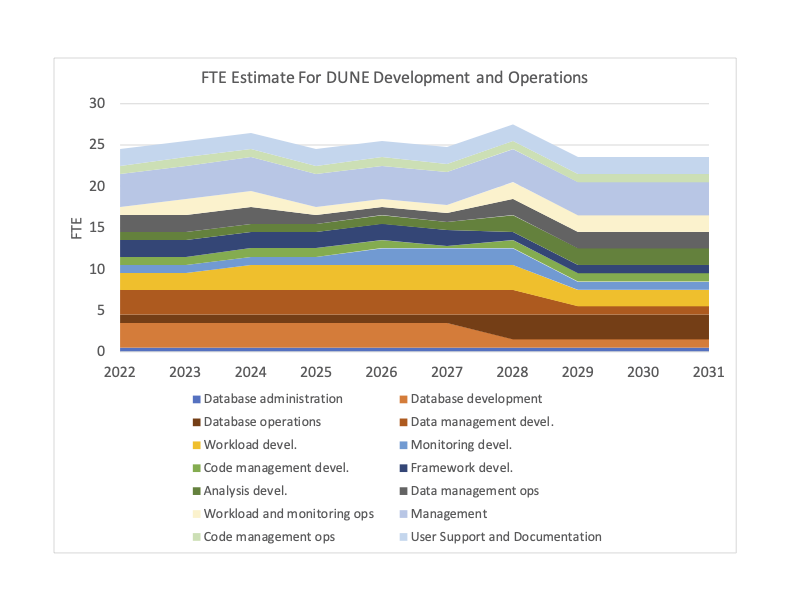
\includegraphics[width=0.9 \textwidth]{graphics/Resources/FTENeeds-2022-02-redo.png}}
\end{dunefigure}
\fixme{HMS - Need to restore the dashed line}
\section{Summary}

This document has described most aspects of \dword{dune} offline computing. Our computing model relies on significant contributions across the collaboration.  

%\section{Computing Contributions Board}

%\hideme{Remove this chapter}
%%%%%%%%%%%%%%%%%%%%%%%%%%%%%%%
%\section{xyz}
%\label{sec:org:xyz}  %% fix label according to section
\end{document}
